% Illustration of the "Stack approach" section of Foucaultgram zone extraction.ipynb.
% Build: tectonic stack_approach.tex, then convert the PDF to SVG (e.g. pdf2svg or PyMuPDF).
\documentclass[border=4pt]{standalone}
\usepackage{amsmath}
\usepackage{tikz}
\usepackage{pgfplots}
\pgfplotsset{compat=1.18}
\usepgfplotslibrary{fillbetween}
\usetikzlibrary{arrows.meta,calc,patterns}

\definecolor{CL}{HTML}{1F77B4} % matplotlib C0, left side (-x)
\definecolor{CR}{HTML}{FF7F0E} % matplotlib C1, right side (+x)
\definecolor{knife}{gray}{0.35}

\tikzset{
  dim/.style={{Latex[length=1.6mm]}-{Latex[length=1.6mm]}, thin},
  ray/.style={thick},
  lbl/.style={font=\small},
}

\begin{document}
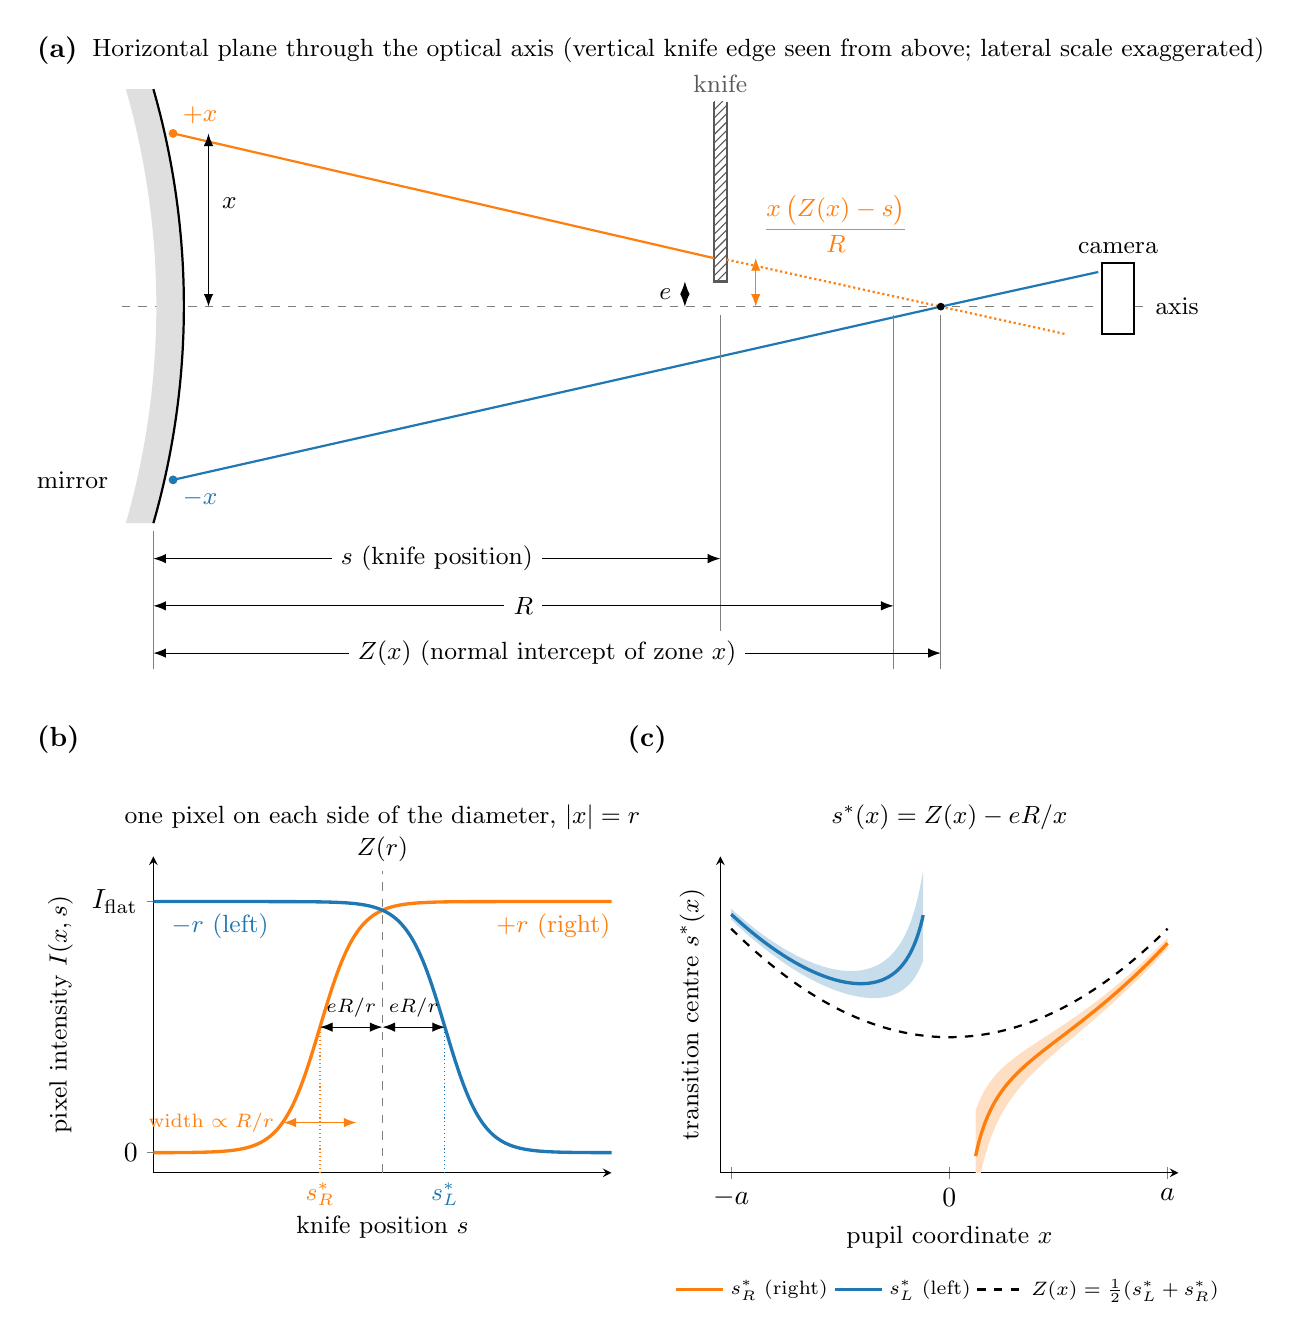
\begin{tikzpicture}[>=Latex]

% ---------------------------------------------------------------- (a) geometry
\begin{scope}
  % R = nominal radius, Z = normal intercept of the zone at height x, s = knife plane
  \def\xz{2.2}   % pupil coordinate x (drawn)
  \def\Zx{10}    % Z(x)
  \def\Rn{9.4}   % R
  \def\s{7.2}    % knife position
  \def\e{0.32}   % knife lateral offset
  \pgfmathsetmacro{\h}{\xz*(\Zx-\s)/\Zx}

  \node[font=\bfseries, anchor=west] at (-1.6,3.25) {(a)};
  \node[lbl, anchor=west, align=left] at (-0.9,3.25)
    {Horizontal plane through the optical axis (vertical knife edge seen from above; lateral scale exaggerated)};

  % optical axis
  \draw[dashed, gray] (-0.4,0) -- (12.6,0) node[right, lbl, black] {axis};

  % mirror
  \fill[gray!25] (0,-2.75) arc[start angle=-16, end angle=16, radius=10] -- ++(-0.35,0)
                 arc[start angle=16, end angle=-16, radius=10] -- cycle;
  \draw[thick] (0,-2.75) arc[start angle=-16, end angle=16, radius=10];
  \node[lbl, anchor=east] at (-0.45,-2.2) {mirror};

  % zone points on the mirror
  \coordinate (PR) at (0.25,\xz);
  \coordinate (PL) at (0.25,-\xz);
  \fill[CR] (PR) circle (1.6pt);
  \fill[CL] (PL) circle (1.6pt);
  \node[lbl, CR, anchor=south west] at (PR) {$+x$};
  \node[lbl, CL, anchor=north west] at (PL) {$-x$};

  % knife blade (enters from the +x side, edge at lateral offset e)
  \fill[pattern=north east lines, pattern color=knife] (\s-0.08,\e) rectangle (\s+0.08,2.6);
  \draw[knife, thick] (\s-0.08,2.6) -- (\s-0.08,\e) -- (\s+0.08,\e) -- (\s+0.08,2.6);
  \node[lbl, knife, anchor=south] at (\s,2.6) {knife};

  % rays: +x is blocked by the knife, -x passes towards the camera
  \draw[ray, CR] (PR) -- (\s-0.08,\h);
  \draw[ray, CR, densely dotted] (\s+0.08,{\xz*(\Zx-\s-0.08)/\Zx}) -- (\Zx,0) -- (11.6,{-\xz*1.6/\Zx});
  \draw[ray, CL] (PL) -- (\Zx,0) -- (12.0,{\xz*2/\Zx});
  \fill (\Zx,0) circle (1.4pt);

  % camera
  \draw[thick, fill=white] (12.05,-0.35) rectangle (12.45,0.55);
  \node[lbl, anchor=south] at (12.25,0.55) {camera};

  % lateral distance of the +x ray at the knife plane
  \draw[dim, CR] (\s+0.45,0) -- (\s+0.45,\h);
  \node[lbl, CR, anchor=west, fill=white, inner sep=1pt] at (\s+0.5,1.05) {$\dfrac{x\,\bigl(Z(x)-s\bigr)}{R}$};
  % knife offset
  \draw[dim] (\s-0.45,0) -- (\s-0.45,\e);
  \node[lbl, anchor=east] at (\s-0.5,{\e/2}) {$e$};

  % pupil coordinate
  \draw[dim] (0.7,0) -- (0.7,\xz);
  \node[lbl, anchor=west] at (0.75,{\xz*0.6}) {$x$};

  % longitudinal dimensions from the mirror vertex
  \foreach \X in {\s,\Rn,\Zx} \draw[thin, gray] (\X,-0.1) -- (\X,-4.6);
  \draw[thin, gray] (0,-2.85) -- (0,-4.6);
  \draw[dim] (0,-3.2) -- (\s,-3.2)   node[midway, fill=white, lbl] {$s$ (knife position)};
  \draw[dim] (0,-3.8) -- (\Rn,-3.8)  node[midway, fill=white, lbl] {$R$};
  \draw[dim] (0,-4.4) -- (\Zx,-4.4)  node[midway, fill=white, lbl] {$Z(x)$ (normal intercept of zone $x$)};
\end{scope}

% ---------------------------------------------------------------- (b) per-pixel transition
  \node[font=\bfseries, anchor=west] at (-1.6,-5.5) {(b)};
  \begin{axis}[
      at={(0,-11.0cm)},
      xlabel style={yshift=-10pt}, width=7.4cm, height=5.6cm,
      xmin=-2.2, xmax=2.2, ymin=-0.08, ymax=1.18,
      axis lines=left, xtick=\empty, ytick={0,1}, yticklabels={$0$,$I_\text{flat}$},
      xlabel={knife position $s$}, ylabel={pixel intensity $I(x,s)$},
      every axis label/.append style={font=\small},
      clip=false, samples=200, domain=-2.2:2.2,
      title={\small one pixel on each side of the diameter, $|x| = r$},
    ]
    % sigmoid model of U; centres s*_R = Z - eR/r, s*_L = Z + eR/r; width ~ R/r
    \addplot[CR, very thick] {1/(1+exp(-(x+0.6)/0.18))};
    \addplot[CL, very thick] {1/(1+exp((x-0.6)/0.18))};
    \draw[dashed, gray] (axis cs:0,-0.08) -- (axis cs:0,1.12) node[above, black, font=\small] {$Z(r)$};
    \draw[densely dotted, CR] (axis cs:-0.6,-0.08) -- (axis cs:-0.6,0.5);
    \draw[densely dotted, CL] (axis cs: 0.6,-0.08) -- (axis cs: 0.6,0.5);
    \node[CR, font=\small, anchor=north] at (axis cs:-0.6,-0.08) {$s^*_R$};
    \node[CL, font=\small, anchor=north] at (axis cs: 0.6,-0.08) {$s^*_L$};
    \draw[dim] (axis cs:-0.6,0.5) -- (axis cs:0,0.5) node[midway, above, font=\scriptsize] {$eR/r$};
    \draw[dim] (axis cs:0,0.5) -- (axis cs:0.6,0.5) node[midway, above, font=\scriptsize] {$eR/r$};
    \draw[dim, CR] (axis cs:-0.95,0.12) -- (axis cs:-0.25,0.12)
      node[pos=0, anchor=east, font=\scriptsize] {width $\propto R/r$};
    \node[CR, font=\small, anchor=west] at (axis cs:1.0,0.9) {$+r$ (right)};
    \node[CL, font=\small, anchor=east] at (axis cs:-1.0,0.9) {$-r$ (left)};
  \end{axis}

% ---------------------------------------------------------------- (c) transition centre across the diameter
  \node[font=\bfseries, anchor=west] at (5.9,-5.5) {(c)};
  \begin{axis}[
      at={(7.2cm,-11.0cm)}, width=7.4cm, height=5.6cm,
      xmin=-1.05, xmax=1.05, ymin=-0.75, ymax=1.0,
      axis lines=left, xtick={-1,0,1}, xticklabels={$-a$,$0$,$a$}, ytick=\empty,
      xlabel={pupil coordinate $x$}, ylabel={transition centre $s^*(x)$},
      every axis label/.append style={font=\small},
      clip=true, samples=150,
      title={\small $s^*(x) = Z(x) - eR/x$},
      legend style={font=\scriptsize, draw=none, fill=white, fill opacity=0.85, text opacity=1,
                    at={(0.5,-0.3)}, anchor=north, legend columns=3},
    ]
    % Z(x) = 0.6 x^2 (arbitrary zonal profile), eR = 0.08, band half-width ~ 0.03/|x|
    \addplot[name path=Ru, draw=none, forget plot, domain=0.12:1] {0.6*x^2 - 0.08/x + 0.03/x};
    \addplot[name path=Rl, draw=none, forget plot, domain=0.12:1] {0.6*x^2 - 0.08/x - 0.03/x};
    \addplot[CR!25, forget plot] fill between[of=Ru and Rl];
    \addplot[name path=Lu, draw=none, forget plot, domain=-1:-0.12] {0.6*x^2 - 0.08/x + 0.03/abs(x)};
    \addplot[name path=Ll, draw=none, forget plot, domain=-1:-0.12] {0.6*x^2 - 0.08/x - 0.03/abs(x)};
    \addplot[CL!25, forget plot] fill between[of=Lu and Ll];
    \addplot[CR, very thick, domain=0.12:1] {0.6*x^2 - 0.08/x};
    \addplot[CL, very thick, domain=-1:-0.12] {0.6*x^2 - 0.08/x};
    \addplot[black, thick, dashed, domain=-1:1] {0.6*x^2};
    \legend{$s^*_R$ (right),$s^*_L$ (left),$Z(x) = \tfrac12(s^*_L + s^*_R)$}
  \end{axis}

\end{tikzpicture}
\end{document}
